\section{MongoDB}
\label{sec:TCH_mongodb}

In this section there will be an overview about MongoDB.

MongoDB is a cross-platform document-oriented database. Classified as a NoSQL database, 
MongoDB eschews the traditional table-based relational database structure in favor of JSON-like documents with dynamic schemas (MongoDB calls the format BSON), making the integration of data in certain types of applications easier and faster. Released under a combination of the GNU Affero General Public License and the Apache License, MongoDB is free and open-source software.

MongoDB was created by Dwight Merriman and Eliot Horowitz, who had encountered development and scalability issues with traditional relational database approaches while building Web applications at DoubleClick, an Internet advertising company that is now owned by Google Inc. According to Merriman, the name of the database was derived from the word humongous to represent the idea of supporting large amounts of data. Merriman and Horowitz helped form 10Gen Inc. in 2007 to commercialize MongoDB and related software. The company was renamed MongoDB Inc. in 2013. 

The database was released to open source in 2009 and is available under the terms of the Free Software Foundation's GNU AGPL Version 3.0 commercial license. At the time of this writing, among other users, the insurance company MetLife is using MongoDB for customer service applications, the website Craigslist is using it for archiving data, the CERN physics lab is using it for data aggregation and discovery and the The New York Times newspaper is using MongoDB to support a form-building application for photo submissions.


\begin {figure}[h]
\graphicspath{{images/chapter_TCH/}}
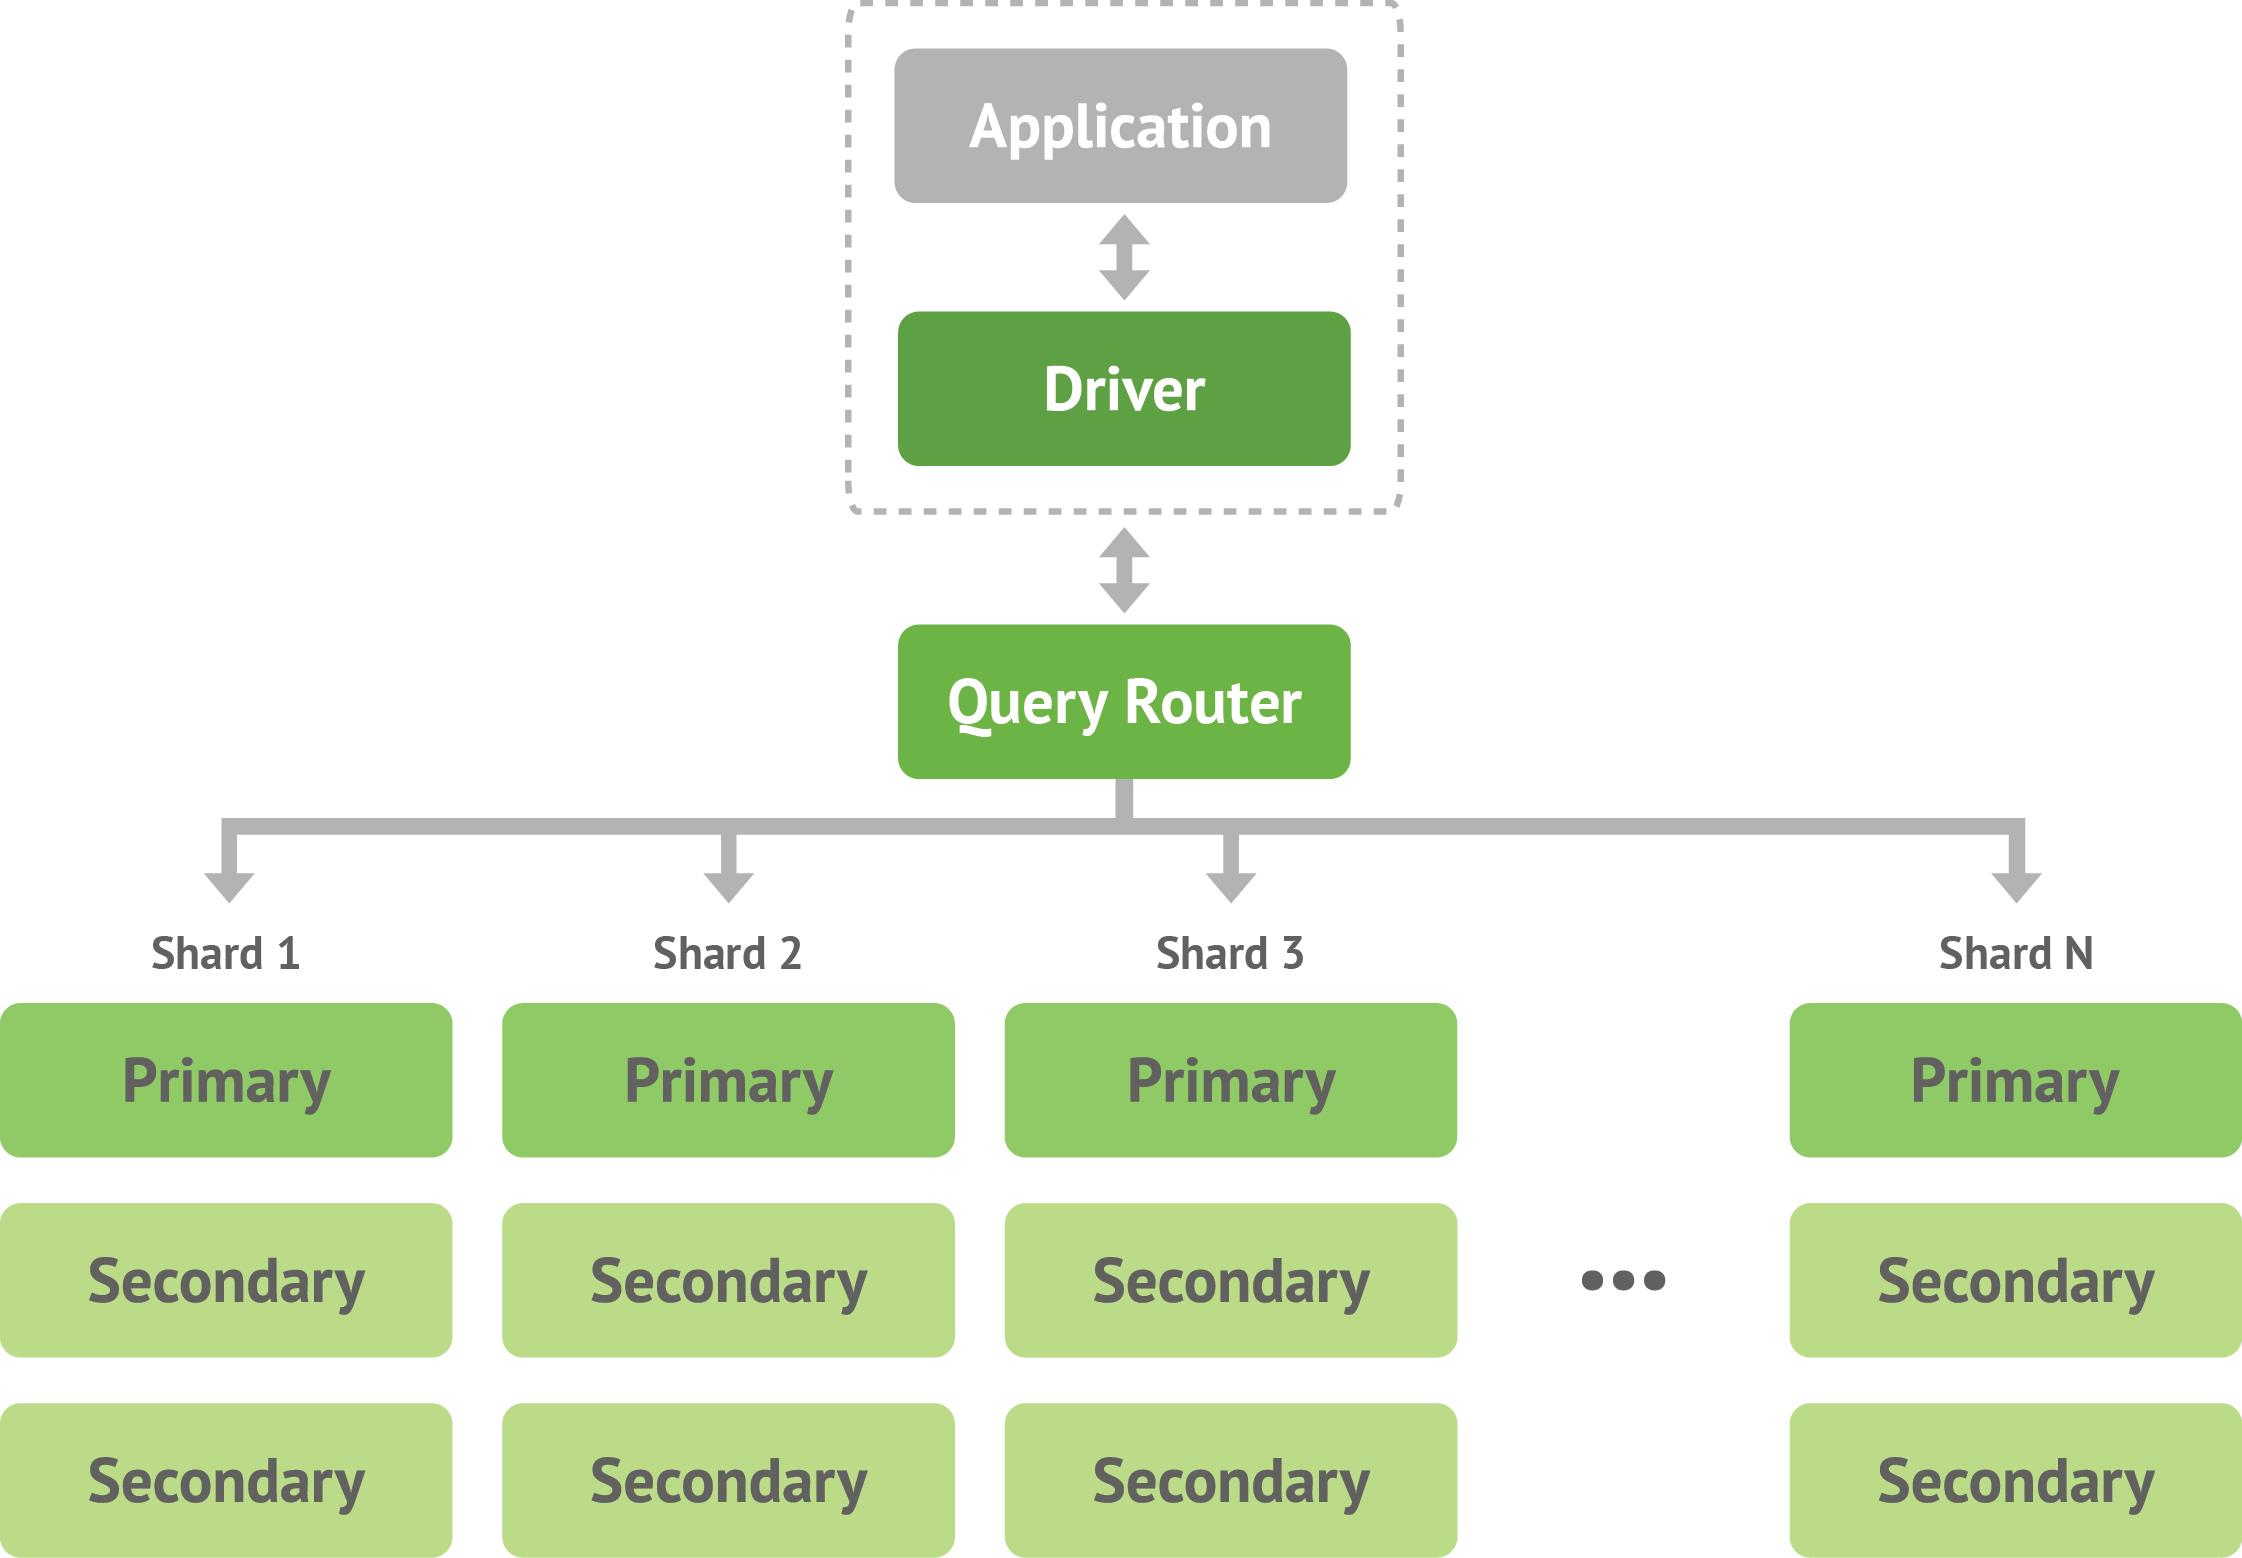
\includegraphics[width=\textwidth]{mongodb_1}
\caption{MongoDB Architecture}
\end {figure}